\documentclass[frontgrid]{flacards}
\usepackage{color}

% For tables with line breaks
\usepackage{tabularx}

% For pictures
\usepackage{graphicx}

% For circuit diagrams
\usepackage{circuitikz}

% For awkward circuit diagrams
\usepackage{tikz}
\usetikzlibrary{shapes}
\usetikzlibrary{arrows}
\usetikzlibrary{circuits}

\definecolor{light-gray}{gray}{0.75}

\newcommand{\frontcard}[1]{\textcolor{light-gray}{\colorbox{light-gray}{$#1$}}}
\newcommand{\backcard}[1]{#1} 

\newcommand{\flashcard}[1]{% create new command for cards with blanks
    \card{% call the original \card command with twice the same argument (#1)
        \let\blank\frontcard% but let \blank behave like \frontcard the first time
        #1
    }{%
        \let\blank\backcard% and like \backcard the second time
        #1
    }%
}

\begin{document}

\pagesetup{2}{4} 

\card{
	What is a hierarchy?
}{
	A hierarchy is a group of objects arranged in tiers of descending magnitude,
	importance or complexity.
}

\card{
	Define {\it digital}.
}{
	An entity that can reside in one of two states at any one time.
}

\card{
	Define {\it analogue}.
}{
	An entity that can reside in an infinite number of possible states.
}

\card{
	How many values can be represented by a binary number containing $n$ bits?
}{
	$2^n$
}

\card{
	Arrange {\tt AND}, {\tt OR} and {\tt NOT} in order of operator precedence.
}{
	{\tt NOT}, {\tt AND}, {\tt OR}
}

\card{
	What is the symbol for {\tt AND}? 
}{
	$\cdot$
	\\
	E.g. $A \cdot B$
}

\card{
	What is the symbol for {\tt OR}?
}{
	$+$
	\\
	E.g. $A + B$
}

\card{
	What is the symbol for {\tt NOT}
}{
	$\overline{\phantom{A}}$
	\\
	E.g. $\overline{A}$
}

\card{
	What is the symbol for {\tt XOR}
}{
	$\oplus$
	\\
	E.g. $A \oplus B$
}

\card{
	What is De Morgan's theorem commonly used for when designing digital 
	circuits?
}{
	Converting gates such as {\tt AND}, {\tt OR}, {\tt XOR} etc into {\tt NAND}
	and {\tt NOR} since they are cheap and fast.
}

\card{
	What is the symbol for an {\tt AND} gate?	
}{
	\begin{circuitikz} \draw
		(0,0) node[and port] (and) {};
	\end{circuitikz}
}

\card{
	What is the symbol for an {\tt OR} gate?	
}{
	\begin{circuitikz} \draw
		(0,0) node[or port] (or) {};
	\end{circuitikz}
}

\card{
	What is the symbol for an {\tt XOR} gate?	
}{
	\begin{circuitikz} \draw
		(0,0) node[xor port] (xor) {};
	\end{circuitikz}
}

\card{
	What is the symbol for an {\tt NOT} gate?	
}{
	\begin{circuitikz} \draw
		(0,0) node[not port] (not) {};
	\end{circuitikz}
}

\card{
	What is the symbol for an {\tt NAND} gate?	
}{
	\begin{circuitikz} \draw
		(0,0) node[nand port] (nand) {};
	\end{circuitikz}
}

\card{
	What is the symbol for an {\tt NOR} gate?	
}{
	\begin{circuitikz} \draw
		(0,0) node[nor port] (nor) {};
	\end{circuitikz}
}

\card{
	What's the symbol for a n:1 multiplexer?
}{
	% I can't find a way to draw it in LaTeX...
	\centering\fbox{
		\begin{minipage}{2in}
			\hfill\vspace{1in}
		\end{minipage}
	}
}

\flashcard{
	What is the truth table for binary addition?
	\begin{tabular}{|c c c|c c|}
		\hline
		$A$ & $B$ & $c_{in}$ & $S$ & $c_{out}$\\ \hline
		0 & 0 & 0 & \blank{0} & \blank{0}\\
		0 & 0 & 1 & \blank{1} & \blank{0}\\
		0 & 1 & 0 & \blank{1} & \blank{0}\\
		0 & 1 & 1 & \blank{0} & \blank{1}\\
		1 & 0 & 0 & \blank{1} & \blank{0}\\
		1 & 0 & 1 & \blank{0} & \blank{1}\\
		1 & 1 & 0 & \blank{0} & \blank{1}\\
		1 & 1 & 1 & \blank{1} & \blank{1}\\ \hline
	\end{tabular}
}

\card{
	How do you negate a binary number?
}{
	1. Invert the bits\\
	2. Add 1
}

\card{
	Convert binary $6$ to $-6$
}{
	1. Start with {\tt 0110}\\
	2. Invert the bits - {\tt 1001}\\
	3. Add 1 - {\tt 1010}
}


\card{
	Which bit is the signed bit when using 2's complement?
}{
	The left most bit.
}

\card{
	How do you subtract two binary numbers?
}{
	1. Invert the number you're subtracting\\
	2. Add 1 to the inverted number\\
	3. Add the number you're subtracting from with the inverted number.\\
	Basically, add the original number to the 2's complement negative of what
	you're taking away.
}

\card{
	What is the {\it sum-of-products}?
}{
	When a number of {\tt AND} gates are {\tt OR}'ed together.
}

\card{
	What is the {\it product-of-sums}?
}{
	When a number of {\tt OR} gates are {\tt AND}'ed together.
}

\card{
	What is the structure of a half adder (in terms of gates)?
}{
	\begin{circuitikz} \draw
	(0,2) node[and port] (and1) {}
	(0,0) node[and port] (and2) {}
	(2,1) node[or port] (or) {}
	(1, -2) node[and port] (and3) {}
	(and1.in 1) node[anchor=east] {$\overline{A}$}
	(and1.in 2) node[anchor=east] {B}
	(and2.in 1) node[anchor=east] {A}
	(and2.in 2) node[anchor=east] {$\overline{B}$}
	(and1.out) -- (or.in 1)
	(and2.out) -- (or.in 2)
	(or.out) node[anchor=west] {S}
	(and3.in 1) node[anchor=east] {A}
	(and3.in 2) node[anchor=east] {B}
	(and3.out) node[anchor=west] {$c_{out}$};
	\end{circuitikz}
}

\flashcard{
	What is the truth table for the half adder?
	\begin{tabular}{|c c |c c|}
		\hline
		$A$ & $B$ & $S$ & $c_{out}$\\ \hline
		0 & 0 & \blank{0} & \blank{0}\\
		0 & 1 & \blank{1} & \blank{0}\\
		1 & 0 & \blank{1} & \blank{0}\\
		1 & 1 & \blank{0} & \blank{1}\\ \hline
	\end{tabular}	
}

\card{
	Define propagation delay.
}{
	Propagation delay is the time taken for the output of a gate to change after
	it's inputs have changed.
}

\flashcard{
	Fill in the table:
	\begin{tabular}{|c|c|}
		\hline
		State & Symbol \\ \hline
		Low      & \blank{0}\\
		High     & \blank{1}\\
		Tristate & \blank{Z}\\
		Unknown  & \blank{X}\\ \hline
	\end{tabular}	
}

\card{
	What does active high and active low mean?
}{
	If a signal is active high, then it is interpreted as {\tt True} when the
	signal is high (e.g. a light is on, or the voltage is positive etc).\\
	If a signal is active low, then it is interpreted as {\tt True} when the
	signal is low (e.g. a light is off, or the voltage is negative etc).
}

\card{
	What are the advantages of a hierarchy:
}{
	1. Encapsulation\\
	2. Reuse of logic\\
	3. Only have to define and test things once
}

\card{
	What is a combinatorial circuit?
}{
	A circuit where the value of the output depends only on the values of the
	input.
}

\card{
	What is a sequential circuit?
}{
	A circuit where the value of the output depends on the values of the input
	and the past history of it's inputs. A sequential circuit requires a clock
	and memory.
}

\card{
	What is a synchronous clock?
}{
	A synchronous clock is one that is effective system wide; all components in
	the system adhere to this clock.
}

\card{
	What is a clock edge?
}{
	The point on a clock signal where the signal is going from low to high 
	(rising or positive edge) or high to low (falling or negative edge.)
}

\card{
	Define bistable.
}{
	An entity that can be in one of two stable states.
}

\card{
	What is a flip flop?
}{
	A bistable device that latches onto a state.
}

\card{
	What is a register made of?
}{
	A series of flip flops, each containing one bit.
}

\card{
	What is a finite state machine?
}{
	A digital system that holds the current state of itself and progresses to a
	new state based on the value of the current state.
}

\card{
	What do {\tt S} and {\tt R} stand for on a S-R flip flop?
}{
	{\tt S} - Set\\
	{\tt R} - Reset
}

\card{
	What is the circuit symbol for a D-type latch?
}{
	\begin{tikzpicture}
		\draw (0,0) rectangle (2,2);
		\draw (0,1.5) -- (-1,1.5);
		\draw (2,0.5) -- (3,0.5);
		\draw (2,1.5) -- (3,1.5);
		\draw (1,0) -- (1,-1);
		\filldraw[fill=white] (2.04, 0.5) circle (1pt);
		\node at (0.2, 1.5) {D};
		\node at (1, 0.2) {En};
		\node at (1.8, 1.5) {Q};
		\node at (1.8, 0.5) {$\overline{Q}$};
	\end{tikzpicture}
}

\card{
	What is the structure of a D-type flip flop?
}{
	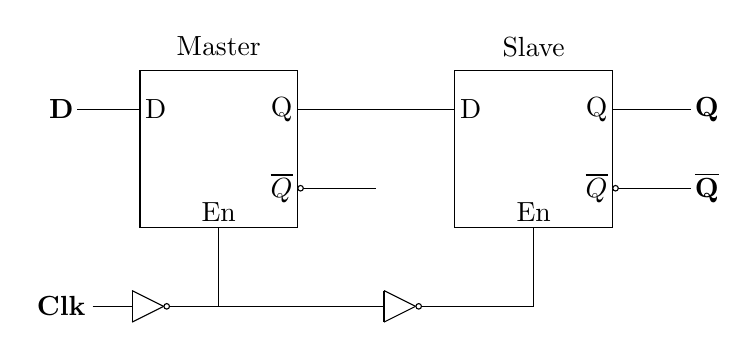
\begin{tikzpicture}
		\draw (0,0) rectangle (2,2);
		\draw (0,1.5) -- (-0.8,1.5);
		\draw (2,0.5) -- (3,0.5);
		\draw (2,1.5) -- (3,1.5);
		\draw (1,0) -- (1,-1);
		\filldraw[fill=white] (2.04, 0.5) circle (1pt);
		\node at (0.2, 1.5) {D};
		\node at (1, 0.2) {En};
		\node at (1.8, 1.5) {Q};
		\node at (1.8, 0.5) {$\overline{Q}$};

		\draw (4,0) rectangle (6,2);
		\draw (4,1.5) -- (3,1.5);
		\draw (6,0.5) -- (7,0.5);
		\draw (6,1.5) -- (7,1.5);
		\draw (5,0) -- (5,-1);
		\filldraw[fill=white] (6.04, 0.5) circle (1pt);
		\node at (4.2, 1.5) {D};
		\node at (5, 0.2) {En};
		\node at (5.8, 1.5) {Q};
		\node at (5.8, 0.5) {$\overline{Q}$};


		% Not gate
		\draw (-0.1,-0.8) -- (-0.1,-1.2);
		\draw (-0.1,-0.8) -- (0.3,-1);
		\draw (-0.1,-1.2) -- (0.3,-1);
		\filldraw[fill=white] (0.34, -1) circle (1pt);
		% Not gate 2
		\draw (3.1,-0.8) -- (3.1,-1.2);
		\draw (3.1,-0.8) -- (3.5,-1);
		\draw (3.1,-1.2) -- (3.5,-1);
		\filldraw[fill=white] (3.54, -1) circle (1pt);
		\draw (-0.6, -1) -- (-0.1, -1);
		\draw (0.38, -1) -- (3.1, -1);
		\draw (3.58, -1) -- (5, -1);

		\node at (-1, -1) {{\bf Clk}};
		\node at (-1, 1.5) {{\bf D}};
		\node at (7.2, 1.5) {{\bf Q}};
		\node at (7.2, 0.5) {{$\overline{\textrm{\bf Q}}$}};

		\node at (1, 2.3) {Master};
		\node at (5, 2.3) {Slave};
	\end{tikzpicture}
}

\card{
	Is a D-type latch level sensitive or edge sensitive? What does that mean?
}{
	The D-type latch is level sensitive, meaning that it will change state 
	whenever the input changes, this means it's {\bf asynchronous}.
}

\card{
	What is the circuit symbol for a D-type flip flop?
}{
	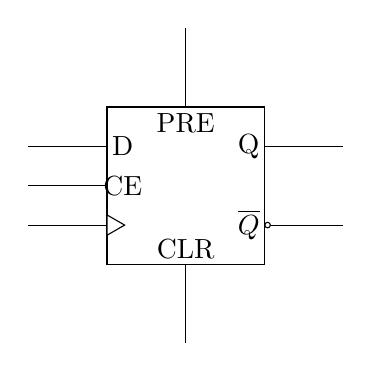
\begin{tikzpicture}
		\draw (0,0) rectangle (2,2);
		\draw (0,1.5) -- (-1,1.5);
		\draw (0,1) -- (-1,1);
		\draw (0,0.5) -- (-1,0.5);
		\draw (2,0.5) -- (3,0.5);
		\draw (2,1.5) -- (3,1.5);
		\draw (1,0) -- (1,-1);
		\draw (1,2) -- (1,3);
		\filldraw[fill=white] (2.04, 0.5) circle (1pt);
		\node at (0.2, 1.5) {D};
		\node at (1, 0.2) {CLR};
		\node at (1, 1.8) {PRE};
		\node at (0.2, 1) {CE};
		\node[fill=white, draw=black, rotate=-90,regular polygon, regular 
			  polygon sides=3,inner sep=1.5pt] at (0.075, 0.5) {};
		\node at (1.8, 1.5) {Q};
		\node at (1.8, 0.5) {$\overline{Q}$};
	\end{tikzpicture}
}

\card{
	What does a D-type flip flop implement to make it synchronous?
}{
	It has an enable switch that can be linked to the clock so that it will
	only change state when the device is clocked.
}

\card{
	What are the three delays in the D-type flip flop?
}{
	The set-up time ($T_{SU}$), the hold time ($T_{H}$) and the
	propagation delay ($T_{PD}$).
}

\card{
	In order to ensure that a D-type flip flop will change state successfully, 
	when does the input have to be constant?
}{
	From the beginning of the set-up time to the end of the hold time.
}

\card{
	What is the propagation delay?
}{
	The time taken for the flip flop to output a change of state.
}

\card{
	What is edge speed?
}{
	The time taken for a signal to change state.
}

% Second book of Paul's notes (pink)

\card{
	What does RTL mean?
}{
	Register Transfer Layer
}

\card{
	Order the following in terms of their level of abstraction from lowest to
	highest:\\
	$\cdot$ Logic Gate Level\\
	$\cdot$ Transistor Level\\
	$\cdot$ Register Transfer Level
}{
	$1$ Transistor Level\\
	$2$ Logic Gate Level\\
	$3$ Register Transfer Level
}

\card{
	What does the CE pin do on a register?
}{
	CE stands for clock enable, and when it is low, the register will ignore 
	clock cycles.
}

\card{
	What are registers made up of?
}{
	Lots of flip flops.
}

\card{
	Define the datapath.
}{
	The datapath is the path of registers and logical functions that the data 
	flows through.
}

\card{
	What does the control block do at the Register Transfer Level?
}{
	The control block controls the operation of the datapath. It sends control 
	signals to the datapath so that the data does indeed, take the right path.
}

\card{
	What data flows between the datapath and the control block?
}{
	The control block gives the datapath control inputs.\\
	The datapath gives control outputs to the control block.
}

\card{
	For a finite state machine with $n$ states, how many flip flops are needed 
	in the register?
}{
	At least $\log_2{n}$
}

\card{
	What is this an example of:\\
	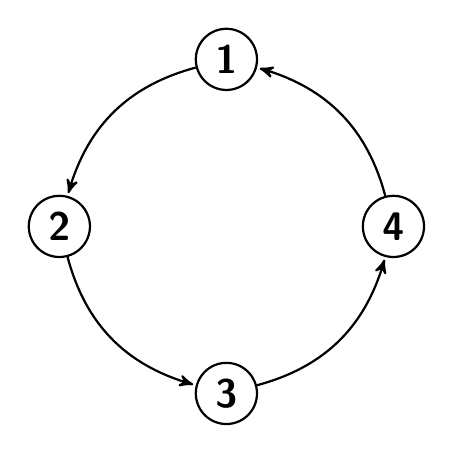
\begin{tikzpicture}[->,>=stealth',shorten >=1pt,auto,node distance=3cm,
                    thick,main node/.style={circle,draw,font=\sffamily\Large\bfseries}]

		\node[main node] (1) {1};
		\node[main node] (2) [below left of=1] {2};
		\node[main node] (3) [below right of=2] {3};
		\node[main node] (4) [below right of=1] {4};

		\path[every node/.style={font=\sffamily\small}]
		(1) edge [bend right] node[left] {} (2)
		(2) edge [bend right] node[left] {} (3)
		(3) edge [bend right] node[right] {} (4)
		(4) edge [bend right] node[right] {} (1);
	\end{tikzpicture}
}{
	A state transition diagram.
}

\card{
	What is the synchronous paradigm?
}{
	When all state changes in a system happen at once (usually at the same time
	as a clock transition).
}

\card{
	What is the formula to subtract $A$ from $B$ using 2's complement?
}{
	$A - B = A + \overline{B} + 1$
}

\card{
	Name the advantages and disadvantages of a FPGA chip.
}{
	\begin{tabularx}{0.48\textwidth}{X}
		{\bf Advantages}\\
		$\cdot$ Don't have to create an actual silicon chip to test hardware designs.\\
		$\cdot$ Far faster than a software hosted simulation.\\
		{\bf Disadvantages}\\
		$\cdot$ Slower operation than a custom chip.\\
		$\cdot$ Requires more power than a custom chip.\\
		$\cdot$ It has a lower capacity than a custom chip (fewer gates can be fit on to
		it).
	\end{tabularx}
}

\card{
	How do you cause a delay of $300ns$ in a Verilog stimulus file? Can you use
	the same command in Verilog files describing hardware?
}{
	{\tt \#300}\\
	You can't use that command in normal Verilog files since there is no way
	for the synthesiser to reliably create a delay of $300ns$ in hardware.
}

\card{
	How do you stop a simulation running in a Verilog stimulus file?
}{
	{\tt \$stop}
}

\card{
	Give some advantages and disadvantages of using a Hardware Description
	Language (HDL).
}{
	\begin{tabularx}{0.48\textwidth}{X}
		{\bf Advantages}\\
		$\cdot$ Is able to express some functions very easily in little code
		(e.g. addition or comparison)\\
		$\cdot$ Will synthesise the gates for you, so you don't have to code the
		logic at the gate level.
		$\cdot$ The code will be easy to read if it's well structured.
		{\bf Disadvantages}\\
		$\cdot$ An inefficient circuit could be synthesised.\\
	\end{tabularx}
}

\card{
	How do you define a module in Verilog?
}{
	\begin{tabular}{l}
		{\tt module <name> (input <input\_1>, \dots, <input\_n>,}\\
		{\tt \phantom{module <name> } output <output\_1>, \dots, <output\_n>);}\\
		{\tt \phantom{  }  //content}\\
		{\tt endmodule}
	\end{tabular}
}

\card{
	Is Verilog case sensitive?
}{
	Yes
}

\card{
	How are numbers formatted in Verilog?
}{
	{\tt <bits>'<base><number>}\\
	e.g. {\tt 4'b1010}, {\tt 8'd255}, {\tt 8'hFF}
}

\card{
	How do you find the complement of a variable in Verilog?
}{
	variable = {\raise.17ex\hbox{$\scriptstyle\sim$}}variable
}

\card{
	What is required if you want to put more than one statement in a Verilog
	block?
}{
	\begin{tabular}{l}
		{\tt begin}\\
		{\tt \phantom{  } statement\_1}\\
		{\tt \phantom{  } \dots}\\
		{\tt \phantom{  } statement\_n}\\
		{\tt end}
	\end{tabular}	
}

\card{
	What are the three forms of assignment in Verilog?
}{
	\begin{tabular}{l l}
		{\bf Name} & {\bf Example}\\
		Continuous & {\tt assign varname = value}\\
		Blocking & {\tt varname = value}\\
		Non-blocking & {\tt varname <= value}\\
	\end{tabular}
}

\card{
	What will Verilog blocks containing continuous assignments synthesise into?
}{
	Combinatorial logic.
}

\card{
	What is the syntax for an in-line conditional statement in Verilog?
}{
	{\tt (cond) ? if\_true : if\_false}
}

\card{
	What types of assignment can go in a always block?
}{
	Either blocking or non-blocking assignments (but not both!).
}

\card{
	What is the syntax for an always block?
}{
	\begin{tabular}{l}
		{\tt always @ (sensitivity\_list)}\\
		{\tt begin}\\
		{\tt \phantom{  } \dots}\\
		{\tt end}
	\end{tabular}	
}

\flashcard{
	Ensure all inputs on the \blank{Right hand side} of statements in an always
	block are in \blank{the sensitivity list}.
}

\card{
	What is the syntax for a Verilog case statement?
}{
	\begin{tabular}{l}
		{\tt always @ (sel, w, x)}\\
		{\tt begin}\\
		{\tt \phantom{  } case(sel)}\\
		{\tt \phantom{    } 0: q = w;}\\
		{\tt \phantom{    } 1: q = x;}\\
		{\tt \phantom{    } default: q = 0;}\\
		{\tt \phantom{  } endcase}\\
		{\tt end}
	\end{tabular}
}

\card{
	How do you define what edge of a signal an always block should be triggered
	on?
}{
	{\tt always @ (posedge clock)}\\
	or\\
	{\tt always @ (negedge clock)}
}

\flashcard{
	Non-blocking assignments happen \blank{simultaneously}.
}

\card{
	In order to produce a FSM in Verilog, what do you write?
}{
	\begin{tabular}{l}
		{\tt always @ (posedge clock)}\\
		{\tt begin}\\
		{\tt \phantom{  }if (reset == 1) state <= 0;}\\
		{\tt \phantom{  }else}\\
		{\tt \phantom{    } case(state)}\\
		{\tt \phantom{      } 0: state = 1;}\\
		{\tt \phantom{      } 1: state = 2;}\\
		{\tt \phantom{      } 2: state = 0;}\\
		{\tt \phantom{      } default: state = 0;}\\
		{\tt \phantom{    } endcase}\\
		{\tt end}
	\end{tabular}
}

\card{
	What does a diagram of a general FSM look like?
}{
	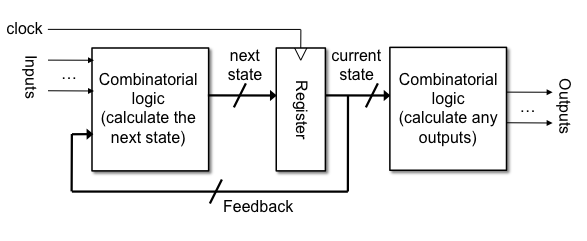
\includegraphics[scale=0.4]{fsm.png}
}

\card{
	What differentiates between an always block that will be synthesised into a
	sequential circuit and one that will be synthesised into a combinatorial
	circuit?
}{
	If the always block has a clock as an input, then it will be sequential.
}

% ==================
% Second half of the course
% ==================

\card{
	State the Amdahl Case rule.
}{
	A balanced computer needs one begabyte of main memory per one begabit per
	second of IO per million instructions per second of CPU performance.
}

\card{
	What are the two types of locality?
}{
	Temporal (if a location is used, then it is likley to be used again soon).\\
	Spatial (if a location is used, then locations around it are likely to be 
	used).
}

\card{
	Describe two characteristics of digital signals that make them useful.
}{
	\begin{tabularx}{0.48\textwidth}{X}
	 - They are composed of two widely seperated states with no intermediate
	 levels.\\
	  - Noise can be eliminated easily because of the seperation of these
	  states.
	\end{tabularx}
}

\card{
	Define latency.
}{
	The time taken for a signal to get from its start to its destination.
	Measured in seconds.
}

\card{
	Define bandwitdh.
}{
	The amount of data that can go through a connection per unit time. Measured
	in bits per second.
}

\card{
	What is clock skew?
}{
	When the wire carrying the clock signal has a different latency to those
	carrying the data signals, so the clock appears to be out of sync with the
	data. It can be mitigated by using a phase shift.
}

\card{
	How is information encoded using Manchester encoding?
}{
	A '1' is encoded as a rising edge, and a '0' is encoded as a falling edge in
	time with the clock tick.
}

\card{
	How is information encoded using non return to zero (NRZI) encoding?
}{
	Any change on a click tick is intrepreted as a 0, and no change is
	intrepreted as a 1. Bit stuffing is used to encode a zero (i.e. a change in
	the signal) if there are six consecutive 1's. This enables the clock signal
	to be extracted from the main signal.
}

\card{
	What are the characteristics of an asynchronous serial communication?
}{
	There is no clock signal transmitted. Both parties agree on the length of
	data packets and an approximate frequency of transmission. Every few bytes,
	they need to re-synchronise their timing to ensure that their clocks do not
	deviate too far apart.
}

\card{
	Describe strobing.
}{
	A seperate wire will carry a strobe signal. This signal will go high when
	data is in a bus ready to be transmitted. When the data has been read, the
	signal will go low indicating the transfer has finished.
}

\card{
	Describe handshaking.
}{
	Handshaking requires two seperate wires; a request line and an acknowledge
	line. When data is to be sent, the requst line goes high and the data
	is then started to be transfered. The acknowledge line goes high while the 
	data is being sent and the request line will go low when the transfer has
	finished, to which the reciever will reply by setting the acknowledge line
	low.
}

\card{
	What is Time Domain Multiplexing?
}{
	TDM is when a connection with high bandwidth is split into many small
	timeframes so that many 'virtual' connections can be established over it.
}

\flashcard{
	What is the truth table for look ahead carry?\\
	\begin{tabular}{|c c|c|}
		\hline
		{\bf A} & {\bf B} & {\bf Cout}\\ \hline
		0 & 0 & \blank{\phantom{0}0\phantom{m}}\\
		0 & 1 & \blank{Cin}\\
		1 & 0 & \blank{Cin}\\
		1 & 1 & \blank{\phantom{0}1\phantom{m}}\\
		\hline
	\end{tabular}
}

\card{
	How do you work out the maximum clock frequency of a processor knowing only
	it's critical path?
}{
	\[
		frequency = \frac{1}{time} = \frac{1}{\textrm{\it cricical path}}
	\]
}

\card{
	What are the three main buses used in computers?
}{
	\begin{tabular}{l}
		- Address bus\\
		- Data bus\\
		- Control bus\\
	\end{tabular}
}

\card{
	Is the bandwidth of a memory cache higher or lower than that of the RAM?
}{
	Higher - it's faster.
}

\end{document} 